\section{Einleitung}


\subsection{Arten von Strahlung}

In diesem Versuch werden $\beta-$und $\gamma-$Zerfälle gemessen.

Diese sind zwei von drei Arten den radioaktiven Zerfalls, die Dritte
Art ist die $\alpha-$Strahlung. Bei der $\alpha-$Strahlung handelt
es sich um Heliumatomkerne, bestehend aus zwei Protonen und zwei Neutronen,
die aus dem radioaktiven Atom hinausgeschleudert werden, dabei nimmt
die Masse des Atoms um vier atomare Masseneinheiten ab (4 atomare
Masseneinheiten=4u$\approx6,64\cdot10^{-27}kg$) und die Ordnungszahl
wird um zwei verringert, dadurch entsteht ein neues Element. Die $\alpha$-
Strahlung besitzt diskrete Energiebeträge.

Da die $\alpha-$Strahlung nicht in diesem Versuch vorkommt, wird
nicht weiter darauf eingegangen.

Bei der $\beta-$Strahlung gibt es zwei mögliche Zerfälle die stattfinden
können. Zum einen der $\beta^{-}$-Zerfall bei dem ein Neutron im
Atomkern zu einem Proton sowie Elektron und einem Neutrino zerfällt,
dabei verbleibt das Proton im Atomkern, das Elektron ist das Teilchen,
welches als $\beta$-Strahlung gemessen werden kann, das Neutrino
ist nur sehr schwer nachweisbar. Neben dem $\beta^{-}$-Zerfall gibt
es noch den $\beta^{+}$-Zerfall bei dem ein Proton in ein Neutron,
ein Positron und ein Neutrino zerfällt, das Positron kann als $\beta$-Strahlung
gemessen werden, auch hier ist das Neutrino nur sehr schwer nachweisbar.

Im Gegensatz zur $\alpha$- und $\gamma$- Strahlung besitzt die $\beta$-
Strahlung keine diskreten sondern kontinuierliche Energiebeträge bis
hin zu einer gewissen Maximalenergie, dieses Phänomen liegt an dem
Neutrino, welches die fehlende Energie aufnimmt.

Die $\gamma$- Strahlung besteht aus hochenergetischen Photonen, den
sogenannten $\gamma$- Quanten, diese entstehen aus angeregten Atomen
dadurch, dass die Protonen und Neutronen im Atomkern ihren Energiezustand
ändern und die Energiedifferenz wird als $\gamma$- Quant ausgesendet,
diese haben wie die $\alpha$- Strahlung diskrete Energiebeträge.


\subsection{Absorption von Strahlung}


\subsubsection{Absorption von $\gamma$- Strahlung}

Bei der Absorption von $\gamma$- Strahlung gibt es drei Absorptionsmechanismen,
dem Photoeffekt bei welchem das $\gamma$-Quant von einem Atom absorbiert
wird und dieses emittiert ein Elektron auf einer der inneren Schalen
der Elektronenhülle. Der zweite Absorptionsmechanismus ist der Comptoneffekt,
bei dem eine inelastische Streuung des $\gamma$- Quants stattfindet,
in welchem es die Frequenz und die Richtung ändert. Der dritte Absorptionsmechanismus
ist die Paarbildung, dort entstehen aus einem $\gamma$- Quant hoher
Energie ( E>2$m_{e}c^{2}\approx 1MeV$) ein Elektron und ein Positron.

Der Absorptionskoeffizient $\mu$setzt sich aus allen drei Absorptionsmechanismen
zusammen
\begin{equation}
	\mu=\mu_{Photo}+\mu_{Compton}+\mu_{Paar}
\end{equation}


diese Größe ist ebenfalls vom Absorbermaterial abhängig.

Treffen nun N $\gamma$- Quanten auf einen Absorber der Dicke \emph{dx
}so wird folgende Relation erhalten
\begin{equation}
	dN=-\mu Ndx
\end{equation}


gelegentlich wird auch die Massenbelegung $\rho$eingeführt, welches
die Dichte des Absorbermaterials darstellt. Dadurch wird $\mu$zu
$\mu_{m}=\frac{\mu}{\rho}$, also 
\begin{equation}
	dN=-\mu_{m}N\rho dx
\end{equation}


durch Integration ergibt sich eine exponentielle Abnahme der Teilchenzahl
mit der Absorberdicke.

\begin{equation}
	N(x)=N_{0}\cdot exp(-\mu)=N_{0}\cdot exp(-\mu_{m}\rho x)
\end{equation}



\subsubsection{Absorption von $\beta-$Strahlung}

Die exponentielle Abnahme gilt nicht für $\beta-$Strahlung, der Grund
hierfür ist, dass die $\beta-$Absorption nicht durch einen einzigen
Prozess erfolgt. Die Elektronen verlieren ihre Energie durch mehrere
inelastische Stöße mit den Atomen des Absorbermaterials, auch ist
es möglich, dass sie durch eine Richtungsänderung aus dem Strahl ausscheiden.
Somit wird für $\beta-$Strahlung die ,,mittlere Reichweite`` $R_{m}$
definiert, dass ist die Absoberdicke bei der noch 50\% der Anfangsstrahlung
vorhanden ist, daneben wird die ,,praktische Reichweite`` definiert,
diese ist als Schnittpunkt des extrapolierten linearen Abfalls der
Reichweitenverteilung mit der Achse \emph{N(x)=0 }definiert.


\subsection{Nachweis der Strahlung}

Zum Nachweis der Strahlung wird ein Geiger-Müller-Zählrohr verwendet.
Im luftdichten Zählrohr befindet sich Argon unter einem Druck von
ungefähr 100mbar und Alkoholdampf, welches einen Partialdruck von
etwa 10mbar hat. Es wird praktisch jedes $\alpha$- und $\beta$-Teilchen
vom Zählrohr erfasst, die $\gamma$- Strahlen werden mit einer kleineren
Menge nachgewiesen.

Im wesentlichen wird der Nachweismechanismus durch eine Ionisierung
eines Argon Atoms, da sich im Inneren des Zählrohrs ein elektrisches
Feld befindet, wird das Ionenpaar, welches aus Elektron und dem Argon-Ion
besteht, jeweils zur Anode bzw. zur Kathode hin beschleunigt. 

Auf diesem Weg ionisieren das Elektron andere Atome und es kommt zu
einer Entladungslawine. Wenn das Argon-Ion auf die Zählrohrwand auftrifft,
werden Sekundärelektronen emittiert, diese tragen zur Erhaltung des
Entladungsprozesses bei. Die Alkoholmoleküle stoppen diesen Entladungsprozess.

Nach jedem Entladungsstoß bleibt das Zählrohr für einige $10^{-4}s$
für neue Teilchen unempfindlich, diese Zeit wird ,,Totzeit`` genannt.
Erst nach diese Zeit kann ein neues Teilchen detektiert werden.


\subsection{Poisson-Verteilung}

Der Erfahrung nach ist die Rate mit der Radioaktive-Zerfälle stattfinden
mit der Poisson-Verteilung beschreibbar. Die Poisson-Verteilung geht
aus der Binomial-Verteilung für eine große Zahl von Objekten und einer
geringen Ereigniswahrscheinlichkeit hervor. Die allgemeine Gleichung
lautet 
\begin{equation}
	\psi_{n}=\frac{\bar{k}^{k}\cdot e^{-\bar{k}}}{k!}\label{eq:Poisson-Verteilung allgemein}
\end{equation}


$\bar{k}$ entspricht dem Erwartungswert 
\begin{equation}
	\bar{k}=np
\end{equation}


$n$ entspricht hier der Anzahl der Atome und $p$ entspricht der
Wahrscheinlichkeit für einen Zerfall.

Bei einer Poisson-Verteilung sind Erwartungswert und Varianz gleich.

\begin{equation}
	\sigma^{2}=np=\bar{k}
\end{equation}


Um nun die Poisson-Verteilung auf den radioaktiven Zerfall anzuwenden
muss der Mittelwert für die gemessenen Zerfälle $\bar{N}$ bestimmt
werden. Dazu werden n-mal die Zahl der zerfallenen Kerne $N_{i}$
jeweils in einem festen Zeitintervall $\triangle T$ gemessen. Dann
wird aus \ref{eq:Poisson-Verteilung allgemein} 
\begin{equation}
	\psi(N)=\frac{\bar{N}^{N}\cdot e^{-\bar{N}}}{N!} \label{eq:pois_id}
\end{equation}


darauf ergibt sich für die mittlere Streuung,
\begin{equation}
\sigma=\sqrt{\bar{N}} \label{eq:std_abw}
\end{equation}


dieses wird $\sqrt{N}-Gesetz$ genannt.

Um  bei den Versuchen einen statistischen Fehler von maximal $ \SI{3}{\percent} $ zu erreichen, darf die Varianz nicht mehr als $ \SI{3}{\percent} $ der Messgröße betragen ($ 1\sigma $ Umgebung $ \sim \SI{68.3}{\percent} $ Sicherheit)
\begin{align}
	&\frac{\sigma}{N} = \frac{\sqrt{N}}{N} = \frac{1}{\sqrt{N}} \stackrel{!}{\leq} \SI{3}{\percent} \notag \\
	\Rightarrow & N \geq \frac{1}{(\SI{3}{\percent})^2} \approx 1112 \label{eq_n_pulszahl}
\end{align}


\newpage
\section{Versuchsteil}
Der Versuchsaufbau ist bei jedem der folgenden Versuche der gleiche. Ausgetauscht werden lediglich die Absorber und die Strahlenquelle. Als Strahlenquelle wird entweder ein \isotope[90]{Sr} $ \beta $-Strahler oder ein \isotope[137]{Cs} $ \gamma $-Strahler verwendet. Auf einen Geiger-Müller-Zähler mit angeschlossenem Zählwerk und Stoppuhr werden die jeweilige Strahlenquelle in vernachlässigbar geringen Abstand ausgerichtet und dazwischen gegebenen Falls die zu prüfenden Absorber platziert. Die gerade nicht verwendeten Strahlenquellen werden gegen die Wand ausgerichtet, um die Messung nach Möglichkeit nicht zu verfälschen.

\subsection{Messung der Zählrohrcharakteristik}
In diesem Versuch ist das Ziel, die Zählrohrcharakteristik zu bestimmen. Das heißt, die Abhängigkeit der gemessenen Strahlenpulse von der am Geiger-Müller-Zähler angelegten zu bestimmen. Dazu wird der zuvor beschriebene Aufbau mit dem $ \beta $-Strahler verwendet und zunächst die höchste Spannung gesucht, bei der keine Strahlung gemessen wird. Daraufhin wird ab etwa $ \SI{50}{\volt} $ über dieser Spannung die Impulsrate gemessen. Um eine statistische Unsicherheit von maximal $ \SI{3}{\percent} $ zu erreichen werden nach \eqref{eq_n_pulszahl} mindestens $ 1112 $ Strahlenpulse gemessen. Beim einstellen der Spannung muss gegebenen Falls beachtet werden, dass die es nicht zur selbständigen Gasentladung kommt und das Zählrohr somit geschädigt wird. Jedoch war es mit unserem Versuchsaufbau nicht möglich, solche Spannungen zu erreichen. \\
Unsere Messwerte sind Tabelle \ref{tab:mess_1} zu entnehmen

\begin{table}[h!]
\begin{tabular}{c|c|c|c|c}
Spannung $ [\si{\volt}] \pm \num{12.5} $ & Impulszahl & Zeit $ [\si{\second}] \pm 1$ & Impulszahl $ [\si{\per\second}] $ & Unsicherheit $ [\si{\per\second}] $ \\ \hline
$ 350 $ & $ 1112 $ & $ 101 $ & $ \num{11.0099} $ & $ \num{0.3477} $ \\
$ 400 $ & $ 1116 $ & $ 103 $ & $ \num{10.8350} $ & $ \num{0.3410} $ \\
$ 450 $ & $ 1117 $ & $ 98 $ & $ \num{11.3980} $ & $ \num{0.3604} $ \\
$ 500 $ & $ 1115 $ & $ 104 $ & $ \num{10.7212} $ & $ \num{0.3373} $ \\
\end{tabular}
\caption{Messwerte Zählrohrcharakteristik}
\label{tab:mess_1}
\end{table}

\subsection{Messung der Untergrundpulse}
\subsection{Häufigkeitsverteilung der Untergrundpulse}
Bei diesem Versuchsteil werden die Untergrundpulse gemessen, die durch natürliche Strahlenquellen auftreten. Der Anfangs beschriebene Versuchsaufbau wird dazu ohne Strahlenquelle und Absorber betrieben. \\
Im ersten Teil dieses Versuches wird $ 100 $ mal die Strahlung in $ \SI{10}{\second} $ gemessen. Wir erhielten die Wahrscheinlichkeitsverteilung gemäß Abbildung \ref{fig:haeuf_hint_1}.

\begin{figure}[h!]
	\centering
	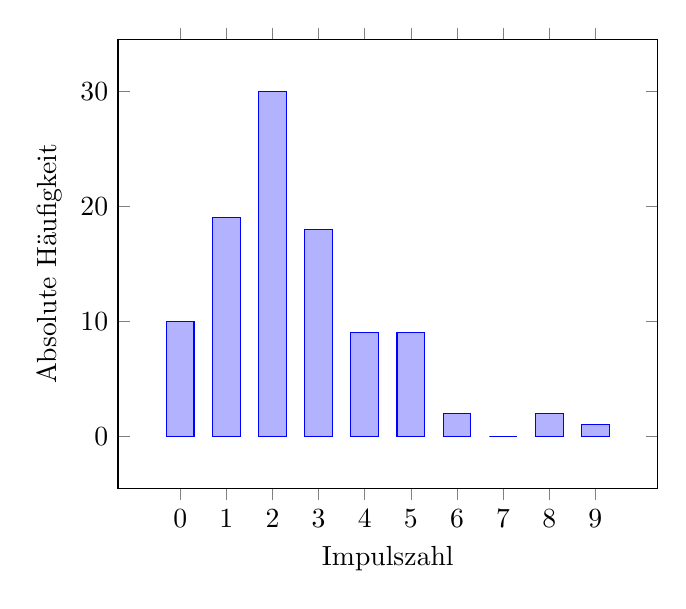
\begin{tikzpicture}
\begin{axis} [
enlargelimits=.15,
ybar,
%symbolic x coords={excellent, good, neutral},
xtick = data,	
xlabel={Impulszahl},
ylabel={Absolute Häufigkeit}
]
\addplot coordinates {(0, 10)
	(1, 19)
	(2, 30)
	(3, 18)
	(4, 9)
	(5, 9)
	(6, 2)
	(7, 0)
	(8, 2)
	(9, 1)
};
\end{axis}
\end{tikzpicture}
	\caption{Häufigkeitsverteilung der Impulszahlen}
	\label{fig:haeuf_hint_1}
\end{figure}

Die mittlere Impulszahl $ \bar N $ ist die Gesamtzahl der Impulse geteilt durch die Anzahl der Messungen. Diese beträgt bei uns $ \bar N = \num{2.51} $. Da von einer Poisson-Verteilung ausgegangen werden kann beträgt die Standard-Abweichung nach \eqref{eq:std_abw} $ \sigma = \sqrt{\bar N} \approx \num{1.585} $.\\
Aus \eqref{eq:pois_id} lässt sich damit die erwartete Wahrscheinlichkeitsverteilung bestimmen. In Abbildung \ref{fig:a2_rech} ist dies gegen die im Experiment ermittelten Häufigkeiten aufgetragen.

\begin{figure}[h!]
\centering
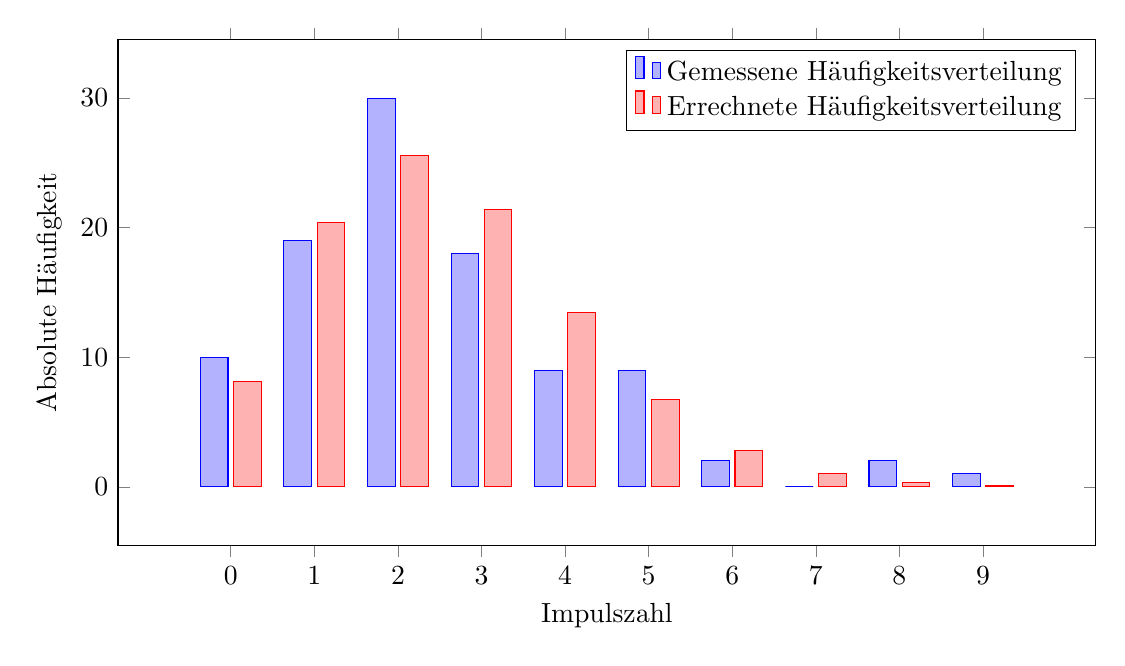
\begin{tikzpicture}[]
\begin{axis} [
width=14cm,
height = 8cm,
enlargelimits=.15,
ybar,
%bar width = 5pt,
%symbolic x coords={excellent, good, neutral},
%nodes near coords,
xtick = data,
xlabel={Impulszahl},
ylabel={Absolute Häufigkeit},
]
\addplot coordinates {(0, 10)
	(1, 19)
	(2, 30)
	(3, 18)
	(4, 9)
	(5, 9)
	(6, 2)
	(7, 0)
	(8, 2)
	(9, 1)
};
\addlegendentry{Gemessene Häufigkeitsverteilung};
\addplot table[x = x, y=y] {
x y
0	8.1268239241
1	20.3983280495
2	25.5999017021
3	21.4185844241
4	13.4401617261
5	6.7469611865
6	2.822478763
7	1.0120602422
8	0.317533901
9	0.0885566768
};
\addlegendentry{Errechnete Häufigkeitsverteilung};
\end{axis}
\end{tikzpicture}
\caption{Rechnerische und gemessene Wahrscheinlichkeitsverteilung der Impulszahlen}
\label{fig:a2_rech}
\end{figure}

\subsection{Korrekturfaktor für Untergrundpulse}
Aus den Untergrundpulsen entsteht für alle anderen Experimente ein Störfaktor, da der Geiger-Müller-Zähler nicht zwischen der Strahlung des Präperats und der Untergrundstrahlung unterscheidet. Um diesen Fehler zu bereinigen wird in diesem Versuchsteil die Untergrundstrahlungsrate ermittelt. Dazu wird die Zeit gemessen, die gebraucht wird um ohne Präperat mehr als $ 500 $ Pulse zu messen.\\
In $ \SI{2070(1)}{\second} $ haben wir $ 501 $ Pulse gemessen. Daraus ergibt sich eine Pulsrate von $ \SI{.2420(108)}{\per\second} $. Diese muss von allen folgenden gemessenen Pulsraten abgezogen werden.

\subsection{Absorbtion von $ \beta $-Strahlung}

\begin{figure}
\centering
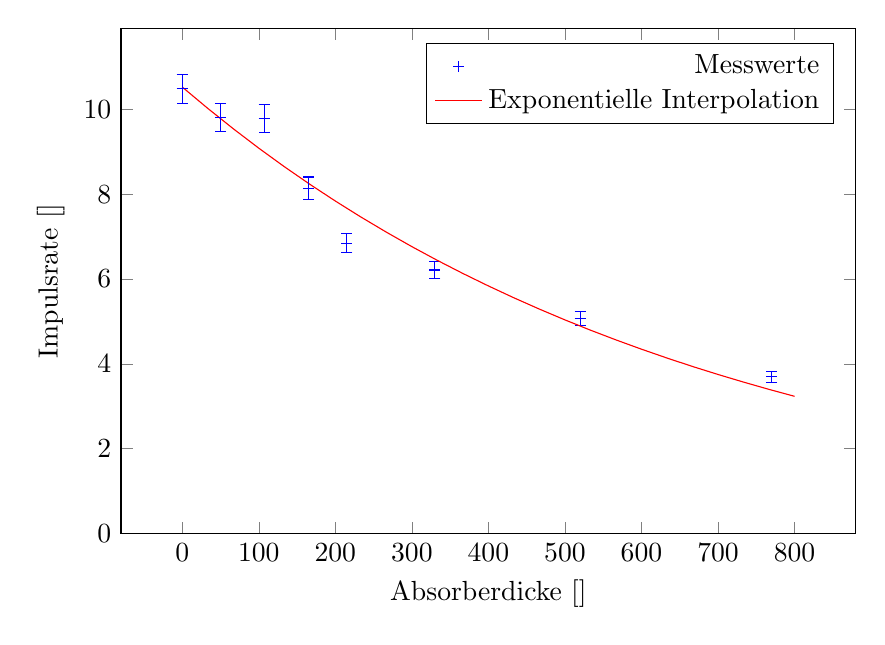
\begin{tikzpicture}
\begin{axis} [
%enlargelimits=.15,
%ybar,
%symbolic x coords={excellent, good, neutral},
%xtick = data,
width=.9\textwidth,
height = 8cm,
error bars/y dir = both,
error bars/y explicit,
%only marks,
ymin = 0,
%ymode=log,
xlabel={Absorberdicke [\si{\micro\meter}]},
ylabel={Impulsrate [\si{\per\second}]},
legend style = {legend pos =  north east, cells={anchor=east}}
]
\addplot+ [mark = +, only marks] table[x = x, y= y, y error = yerror]  {
x	y	yerror
0	10.4791248606	0.3480304704
50	9.8030160595	0.3249560292
107	9.7847567288	0.3231269543
165	8.1339108641	0.2695473226
215	6.847142989	0.228052825
330	6.211994003	0.206946066
520	5.0722567288	0.171892932
770	3.6943667742	0.1295697446
};
\addlegendentry{Messwerte};
\addplot+[no marks, domain=0:800] {10.52378637*exp(-1474.24606886e-6*x)};
\addlegendentry{Exponentielle Interpolation};
\end{axis}
\end{tikzpicture}
\caption{Absorberdicke-Pulsrate-Diagramm für Aluminium mit linearer Skala}
\end{figure}

\begin{figure}
\centering
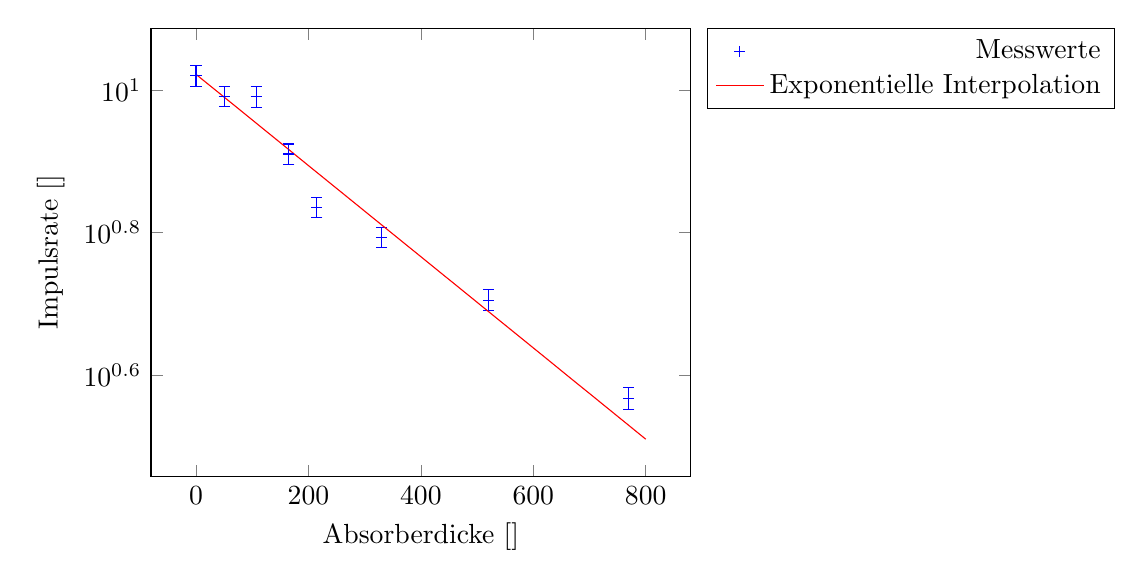
\begin{tikzpicture}
\begin{axis} [
%enlargelimits=.15,
%ybar,
%symbolic x coords={excellent, good, neutral},
%xtick = data,
error bars/y dir = both,
error bars/y explicit,
%only marks,
%ymin = 0,
ymode=log,
xlabel={Absorberdicke [\si{\micro\meter}]},
ylabel={Impulsrate [\si{\per\second}]},
legend style = {legend pos = outer north east, cells={anchor=east}}
]
\addplot+ [mark = +, only marks] table[x = x, y= y, y error = yerror]  {
x	y	yerror
0	10.4791248606	0.3480304704
50	9.8030160595	0.3249560292
107	9.7847567288	0.3231269543
165	8.1339108641	0.2695473226
215	6.847142989	0.228052825
330	6.211994003	0.206946066
520	5.0722567288	0.171892932
770	3.6943667742	0.1295697446
};
\addlegendentry{Messwerte};
\addplot+[no marks, domain=0:800] {10.52378637*exp(-1474.24606886e-6*x)};
\addlegendentry{Exponentielle Interpolation};
\end{axis}
\end{tikzpicture}
\caption{Absorberdicke-Pulsrate-Diagramm für Aluminium mit log Skala}
\end{figure}